\section{Source audit, reproducibility, and further research}
\label{audit:sec}

\subsection{What should change in the project status}

Table~\ref{audit:tab:status} records the precise scope of the proved
changes. The integration notes name the source paths and incoming
archive members. They are proposals for integration; the source
repository has not been modified.

\begin{table}[tbp]
\centering\small
\renewcommand{\arraystretch}{1.2}
\begin{tabular}{@{}>{\raggedright\arraybackslash}p{0.28\textwidth}>{\raggedright\arraybackslash}p{0.33\textwidth}>{\raggedright\arraybackslash}p{0.31\textwidth}@{}}
\toprule
Source target & Result established here & Scope that remains open\\
\midrule
Rational tetralogarithm,
\src{golden:eq:tetra} &
Exact proof, Theorem~\ref{rattetra:thm:main};
the equivalent cross-base form follows &
Minimal certificate size and reduction to named classical
specializations\\
Incoming \src{conj:euler-rate} &
Matching asymptotic, second scale, and maximizing-order displacement,
Theorem~\ref{lateaxis:thm:sharpasymptotic} &
Effective error constants and the full smaller-index optimization\\
Fractional continuation of integer Euler tails &
Compensated exact kernel and both logarithmic sequences,
Theorems~\ref{frac:thm:kernel} and \ref{frac:thm:allorders} &
Joint endpoint regimes and optimal truncation of divergent series\\
Fixed-total late-error comparison &
All-$N$ domination for $a\ge1$; a unique reversal for $0<a<1$,
Theorems~\ref{phasefrac:thm:above} and \ref{phasefrac:thm:unique} &
Quantitative dependence of the crossing order on $a,b$\\
Effective Lerch saturation &
$O(n^6\log^2 n)$ sufficient order and a power-sized index range,
Theorem~\ref{polylerch:thm:saturation} &
Least saturation order and optimal polynomial root separation\\
\bottomrule
\end{tabular}
\caption{Status changes relative to the pinned ProveIt source.
Each row distinguishes a proved statement from a sharper question.}
\label{audit:tab:status}
\end{table}

The rational tetralogarithm identity should now be designated a
theorem with an exact certificate. The two duplication formulas
already in the manuscript make the displayed cross-base relation
equivalent, so its status changes at the same time. This does not
establish uniqueness among all rational tetralogarithm relations.
Nor should the higher golden formulas be promoted merely because
the weight-four certificate is successful.

For the Euler problem, the incoming lower asymptotic was already
proved~\cite{incoming-bounds}. The new work supplies the missing
uniform upper argument, an exact eventual reduction, and more precise
asymptotics. The large numerical threshold in the reduction is
part of the theorem's explicit scope. The unique maximum and its
strictly increasing location on the axis hold at every $N\ge2$;
strict decrease of the global $C_N$ is proved here only in the
eventual range.

The new Lerch estimate improves a sufficient bound. It does not
change the meaning of the least uniform simplicity threshold.
The exact finite calculations concern auxiliary polynomials with
rational coefficients, while the all-index theorem concerns
reciprocal-gamma Appell polynomials with transcendental coefficients.
The transfer between them is the proved mesh-preserving gamma-product
limit, not a numerical comparison of their roots.

\subsection{A correction and three important proof distinctions}

The passage adjoining \src{vertical:eq:Im3} in
\src{03-algebraic.tex} describes the imaginary part of
$\Li_3(1+i)$ as no longer elementary. The displayed representation
through a hypergeometric constant does not prove such a
nonreducibility assertion. A precise replacement is:
\begin{quote}
The transformations displayed here do not reduce the imaginary part
to the elementary constants used here; the following formula expresses
it through the central-binomial Gaussian tower constant.
\end{quote}
The accompanying patch makes this limited wording correction and
preserves the displayed identity. A proof of arithmetic
nonreducibility would require a different theorem.

Three other distinctions matter for integrating the new material.
First, the compensated density at $a+b<1$ does not contradict the
source's finite signed-measure obstruction. The primitive and density
are tested against functions that vanish at zero. A possible critical
endpoint atom is therefore invisible, and the ordinary alternating
boundary series is not being used in a region where it diverges.

Second, retaining only the total-order logarithmic sequence would
omit the term
\[
 -\frac{b\zeta(b+1)\sqrt\pi}{2\Gamma(a-1)}
 N^{-1/2}L^{a-2}.
\]
For $0<b<1$, it occurs between two successive integer inverse-log
orders. The real-order extension must retain both sequences.
When $b=m$ is integral and $a$ is not, the combined coefficients
grow as $\Gamma(j-a)$; the exact gamma index is significant for
optimal-truncation work.

Third, formal relation spaces and numerical period spaces are
different objects. The incoming work contains exact nonmembership
statements for specified finite collections of shuffle or auxiliary
relations~\cite{incoming-uniform}. Such statements can certify that
one proposed derivation is insufficient. They do not exclude all
functional identities, and they do not prove arithmetic independence
of the evaluated constants. The Gaussian conjectures
$S_6,S_8,S_{10},S_{12}$ remain unresolved by this article.

\subsection{Exact checks and numerical illustrations}

The exact replay for the tetralogarithm theorem reconstructs the
rational functions from the forty-two rows, factors every $1-f_i$,
checks the factorizations by multiplication, and cancels all $230$
touched tensor coordinates. It retains the rational prime $2$.
Discarding rational contents would change the vector space and
invalidate the proof. The verifier also checks the endpoint
polynomial, the original six arguments and coefficients, the
one-parameter formula, and the $t=1/3$ specialization.

At points where an auxiliary factor vanishes, the descent functional
is defined by its values on independent generators and then extended
linearly. It is not defined by evaluating a logarithm of that
vanishing factor. Likewise, a term involving $\ell_1(1)$ is removed
only after its coefficient has been proved zero. These two details
are included in the proof and replay because overlooking either
would produce an invalid symbolic calculation.

The fractional verifier checks all $64$ integer-density
specializations with $1\le a,b\le8$, along with eight coefficient
groupings. Its interval engine encloses the half-order comparisons
using only integer square roots and rational arithmetic. The
dedicated threshold replay uses that same engine and records its
dependency explicitly. It certifies the two signs needed to locate
the unique transition.

The Lerch replay verifies the auxiliary polynomial identity at
$2\le n\le16$ and isolates all $135$ roots in exact rational
brackets. It checks simplicity, additive and logarithmic gap
inequalities, $90$ finite-multiplier coefficient identities, and
seven exact gamma-moment inequalities. These finite checks support
normalization and give useful improved thresholds, but the
all-index theorem follows from the analytic proof.

\begin{figure}[tbp]
\centering
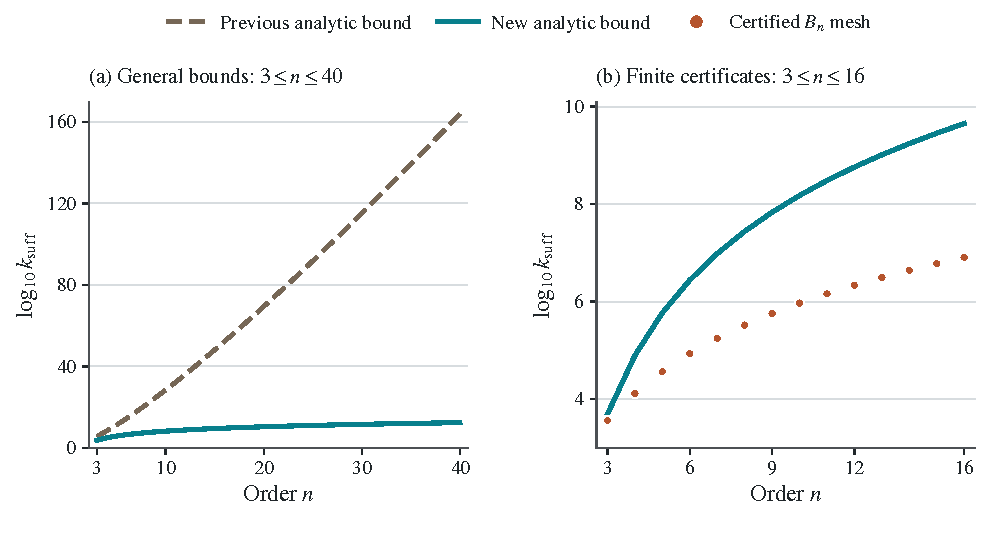
\includegraphics[width=\textwidth]{figures/lerch_thresholds.pdf}
\caption{Uniform sufficient bounds for Lerch zero saturation.
Panel (a) compares the earlier
$576n^2(3n)^{2n-4}$~\cite{incoming-uniform} with the new
$\mathcal K_n$ from \eqref{polylerch:eq:threshold}.
Panel (b) compares $\mathcal K_n$ with the smaller bounds obtained
from exact certified meshes of $B_n$. The vertical coordinates are
base-ten logarithms. Every displayed quantity is a sufficient bound;
no sharpness assertion is made.}
\label{audit:fig:thresholds}
\end{figure}

The Euler diagnostic program checks the derivative polynomials
symbolically and evaluates the positive integral remainder
$M_N(b)$ at high precision. Table~\ref{audit:tab:axis} illustrates
the axis optimization; its numbers are numerical approximations,
not interval-certified maximizers.

\begin{table}[tbp]
\centering\small
\begin{tabular}{@{}rrrr@{}}
\toprule
$N$ & Axis maximizer $b_N$ & $A_N-1$ & $N^p(A_N-1)$\\
\midrule
2 & $3.239719039892$ & $3.9230434864\,10^{-2}$ & $0.12830$\\
10 & $6.746559248034$ & $3.2851480198\,10^{-3}$ & $0.16829$\\
100 & $12.331892789531$ & $6.8858193177\,10^{-5}$ & $0.18071$\\
$10^4$ & $23.792066269001$ & $2.5107487089\,10^{-8}$ & $0.17292$\\
$10^{12}$ & $69.281926034579$ & $5.1420139643\,10^{-22}$ & $0.167984320879$\\
\bottomrule
\end{tabular}
\caption{Numerical axis optimization using the positive centered
integral. Full working values are supplied in
\src{data/late_euler_optimizers.csv}. Only the last row lies beyond
the explicit global axis-reduction threshold.}
\label{audit:tab:axis}
\end{table}

The second asymptotic scale converges much more slowly than the
leading normalized maximum. For example, at the leading maximizing
location $B\log N+d_0$, the diagnostic
$N^I\sqrt{\log N}\,M_N$ is still approximately $1.45355$ at
$N=10^{10000}$, whereas its proved limit is
$D=1.56777020071\ldots$. The small exponent
$4-(2B-1)=5-2B>0$ in the limiting positive tail explains why
the dominated-convergence proof can coexist with this slow approach.
The second term should therefore not be substituted into a rigorous
finite-$N$ error budget without an additional effective remainder
estimate.

\subsection{Further research questions and concrete conjectures}

\paragraph{1. A shorter tetralogarithm derivation.}
Can the forty-two-row tensor certificate be decomposed into a small
number of standard Kummer functional-equation substitutions?
This would make the proof easier to recognize in the classical
literature. The exact relation is established already; minimality
is a separate optimization problem. A systematic library of
real-branch descent certificates should record rational prime
contents, argument factorizations, endpoint values, and permitted
crossings.

\paragraph{2. Higher-weight golden and Gaussian identities.}
Apply the certificate method to the specific higher golden
reconstructions, with their endpoint logarithms and higher-weight
compatibility conditions made explicit. For the Gaussian problem,
seek an exact certificate for $S_6$ before enlarging the conjectural
$S_{2m}$ family. A useful success criterion is an explicit rational
relation in a stated functional-equation space whose analytic
evaluation can be proved. A smaller numerical residual or formal
rank calculation alone does not meet that criterion.

\paragraph{3. Is global axis reduction valid at every later index?}
The following strengthens the eventual theorem:
\begin{conjecture}[Axis reduction at every $N\ge2$]
\label{research:conj:allaxis}
For every integer $N\ge2$,
\[
 \sup_{a,b>0}R_N(a,b)=\max_{b>0}R_N(0,b).
\]
Every positive outer order gives a strict inequality.
\end{conjecture}
The axis maximum and its uniqueness are already proved for each such
$N$. What is missing is a global comparison over the positive
quadrant at the smaller indices. A proof need not show that
$R_N(a,b)$ decreases in $a$ for every $a,b$: that stronger
pointwise statement is not used by the present argument.
Validated compact optimization, joined to analytic estimates on all
noncompact parameter regions, could also reduce the explicit
threshold substantially.

\paragraph{4. Effective second-scale asymptotics and near maximizers.}
Obtain an explicit error estimate for
\eqref{lateaxis:eq:second}, and develop the inverse-$\log N$
corrections multiplying $N^{-I}/\sqrt{\log N}$. The centered
integral suggests coefficients involving derivatives of
$\Gamma(1/2-B)$. One must control the positive tail uniformly
before integrating an expanded density. Determine also the
sharp scale of the outer order among near maximizers; the proved
bound in Corollary~\ref{lateaxis:cor:concentration} is a necessary
concentration estimate, not an optimal local expansion in $a$.

\paragraph{5. The reversal order near outer order one.}
For each fixed $b>0$, the theorem implies
$\nu(a,b)\to\infty$ as $a\uparrow1$. Balancing the generic
$N^{-1/2}$ difference and the critical $N^{-1}$ difference leads
to the following precise candidate.
\begin{conjecture}[Near-critical reversal scale]
\label{research:conj:crossing}
For fixed $b>0$, with $\varepsilon=1-a\downarrow0$,
\[
 \nu(1-\varepsilon,b)\sim
 \frac{\bigl(\log(1/\varepsilon)\bigr)^{2b+2}}
 {\pi b^2\Gamma(b+1)^2\zeta(b+1)^2\,\varepsilon^2}.
\]
\end{conjecture}
The heuristic balance is
\[
 \varepsilon b\zeta(b+1)\sqrt\pi\,\Gamma(b+1)\sqrt N
 \asymp L^{b+1},\qquad L=\tfrac12\log N.
\]
It uses $1/\Gamma(-\varepsilon)\sim-\varepsilon$ and
$L\sim\log(1/\varepsilon)$ at the proposed crossing.
This is a newly proposed asymptotic, not a consequence of exchanging
limits in the fixed-parameter theorems. A proof needs a joint
expansion that retains both terms uniformly as $a\uparrow1$.
Quantitative asymptotics for the derivative zero sequence
$\nu_r$ from Corollary~\ref{phasefrac:cor:derivatives} form a
related problem.

\paragraph{6. Optimal truncation and exponentially small Euler terms.}
For integral $b=m$ and nonintegral $a$, the coefficient law
\eqref{frac:eq:largecoefficient} identifies the factorial growth
of the logarithmic series. Determine the optimal truncation index,
a rigorous remainder near that index, and its relation to the
exponentially small density terms discarded in the algebraic
large-$T$ expansion. Near integral $a$, the factor $\sin(\pi a)$
vanishes; any uniform result must resolve the transition from a
divergent expansion to an exactly terminating one.

\paragraph{7. Better Appell mesh and the least Lerch threshold.}
Can the explicit $n^{-3}$ gap be improved to $cn^{-2}$, or to
a different optimal scale? The auxiliary factor
$R_n(x)=\sum e_r x^r/(r+1)!$ provides a rational route to this
question. A stronger uniform mesh estimate immediately improves
the sufficient derivative order through
$\lceil(16+24H_{n-1}/\delta_n)^2\rceil$.
The elementary endpoint gives the necessary condition
$k\ge n-1$ for uniform simplicity; determine whether that condition
is also sufficient. It is important to separate saturation in
number from simplicity at the endpoint $\rho=0$.

\paragraph{8. Signed concentration and uniform higher zero offsets.}
The present proof controls an absolute logarithmic moment and gives
relative error $O(k^{-1/2})$. Cancellations in signed moments should
permit sharper location estimates. Develop them while $n$ grows
with $k$ and $\rho$ ranges over the full closed interval. Fixed-index
offset formulas in the manuscript are useful starting points, but
their constants must be controlled with respect to $n$ before a
growing-index conclusion is drawn.

